\documentclass[a4paper, oneside]{csthesis}

% package to be able to use special characters
\usepackage[utf8]{inputenc}

% Sophisticated math package
\usepackage{amsmath}

% Special symbols
\usepackage{amssymb}

% nicely render theorems and proofs
\usepackage[standard,thmmarks,amsmath]{ntheorem}

\usepackage{graphicx}

% package to format pseudo-code. Check the package documentation.
% http://ctan.org/pkg/listings
\usepackage{algorithmic}
\usepackage{algorithm}

% awesome code highlighting and coloring for many languages
% http://en.wikibooks.org/wiki/LaTeX/Packages/Listings
\usepackage{listings}
\lstset{language=Java}

% Provides \xspace command that evaluates to a space if the next character in the source is a blank and
% no space if next character is no blank. Useful in command definitions.
\usepackage{xspace}

% Provides a more flexible tabular environment
\usepackage{tabularx}

% Enables the use of the H location specifier for float environments that puts the float exactly where it is located in the source.
\usepackage{float}

% Enables the use of colours
\usepackage{color}

\usepackage{paralist}

% nice string commands
\usepackage{xstring}

\usepackage{colortbl}
\usepackage[table]{xcolor}

% wide tables
\usepackage{adjustbox}

\definecolor{DarkGray}{gray}{0.7}
\definecolor{Gray}{gray}{0.9}

\definecolor{darkblue}{rgb}{0,0,.5}
% Enables clickable links in the PDF and additional PDF specific configuration options.
\usepackage[
            colorlinks=true,
            linkcolor=darkblue, urlcolor=darkblue, citecolor=darkblue,
						raiselinks=true,
            bookmarks=true,
            bookmarksopenlevel=1,
            bookmarksopen=true,
            bookmarksnumbered=true,
            hyperindex=true,
            plainpages=false,
            pdfpagelabels=true,
            pdfstartview=FitH,
            pdfstartpage=1,
            pdfpagelayout=OneColumn
            ]{hyperref}

% Provides a highly configurable way to create references inside the document and automatically prefix
% the number reference by fig./eq./chapter and so on. You only have to use \cref{label} or \Cref{label}
% to obtain "Lemma 4.1" or "Corollary 4.1" etc., depending on the label. See an example in the proof
% of the first theorem or check the documentation of the package for further information.
\usepackage[noabbrev]{cleveref}


% awesome figure placment
\usepackage{subfigure}

% Load own command definitions, a few helpful ones are already defined there.

% This alters the numbering of theorems and lemmas.
\theoremsymbol{\ensuremath{\scriptstyle \Diamond}}
\renewtheorem{theorem}{Theorem}[chapter]
\renewtheorem{lemma}[theorem]{Lemma}
\renewtheorem{corollary}[theorem]{Corollary}
\renewtheorem{definition}[theorem]{Definition}

% This creates a two new theorem-like environments
\theoremsymbol{}
\newtheorem{notation}[theorem]{Notation}
\theorembodyfont{}
\newtheorem*{problem}{Problem}

\crefname{algorithm}{algorithm}{algorithms}
\Crefname{algorithm}{Algorithm}{Algorithms}

% This changes the comment style of the "algorithmic" pseudocode package
\renewcommand\algorithmiccomment[1]{\hfill \small \(\triangleright\) #1}

% This creates four commands to leave annotations in your document
\newcommand{\TODO}[1]{\noindent {{\color{red}\fbox{\sffamily \bfseries TODO}} \sffamily #1}}
\newcommand{\FIXME}[1]{\noindent {{\color{green}\fbox{\sffamily \bfseries FIXME}} \sffamily #1}}
\newcommand{\CONSIDER}[1]{\noindent {{\color{blue}\fbox{\sffamily \bfseries CONSIDER}} \sffamily #1}}
\newcommand{\RW}[1]{\noindent \color{blue}#1}

% This creates a command to easily refer to websites as footnotes
\newcommand{\websource}[3]{\footnote{{#1\newline Available at: #2 [Accessed
#3]}}}

\newcommand\telesto{\textit{Telesto}}

\graphicspath{{figures/}}

% style whole rows in table
\usepackage{array}
\newcolumntype{$}{>{\global\let\currentrowstyle\relax}}
\newcolumntype{^}{>{\currentrowstyle}}
\newcommand{\rowstyle}[1]{\gdef\currentrowstyle{#1}%
  #1\ignorespaces
}


%%%%%%%%%%%%%%%%%%%%%%%%%%%%%%%%%%%%%%%%%%%%%%%%%%%%%%%%%%%%%%%%%%%%%%%%%%%%%%%%%%%%%%%%%%%%%%%%%
% DOCUMENT METADATA

\thesistype{Report Group 32}
\title{Telesto - A Distributed Message Passing System}

\author{Dominic Langenegger, Simon Marti}
\email{\{dominicl,simarti\}@student.ethz.ch}
\institute{Advanced Systems Lab 2013 \\[2pt]
Systems Group \\[2pt]
ETH Zürich}

% You can put in your own logo here "\includegraphics{...}" or just comment the command
% \logo{}

\supervisors{Markus Pilman\\[2pt] Prof.\ Dr.\ Gustavo Alonso}

% You can comment the following two commands if you don't need them
\keywords{}
%\categories{ACM categories go here.}

\date{November 15, 2013}

%%%%%%%%%%%%%%%%%%%%%%%%%%%%%%%%%%%%%%%%%%%%%%%%%%%%%%%%%%%%%%%%%%%%%%%%%%%%%%%%%%%%%%%%%%%%%%%%%

\begin{document}

\frontmatter
\maketitle % do not remove this line

\cleardoublepage

%\begin{acknowledgements}
%\end{acknowledgements}


\begin{abstract}
	This document describes \telesto, a distributed message passing system
	built as mandatory course work for the course {\it Advanced Systems Lab} at ETH
	Zurich in autumn semester 2013.
	
	
	
	\TODO{final findings}
\end{abstract}

\tableofcontents

\mainmatter % do not remove this line

% Start writing here
\chapter{Introduction}
	


\chapter{Goals}

	
\chapter{Architecture}
    This chapter explains the basic architecture of \telesto{} explaining how each
    part of the system works and how they communicate together.
    \Cref{ch:implementation} gives a more detailed insight about how the
    implementation of some important component looks like.

    \telesto{} is a three tier system:
    \begin{description}
        \item[Database] \ \\
            A {\it PostgreSQL}~\websource{PostgreSQL
            Website}{http://www.postgresql.org/}{November 15, 2013} database storing the persistent state of the system
        \item[Middleware] \ \\
            The part that provides many clients simultaneously with services of
            the message passing system and stores all data in the database. This
            part can be easily replicated.
        \item[Client] \ \\
            Clients that pass and receive messages from the system by talking to
            one middleware instance.
    \end{description}

    Figure~\cref{fig:telesto-architecture} shows a sample architecture diagram.
    It is important to note, that clients only talk to middlewares and only a
    middleware has direct access to the database.

    \begin{figure}[h]
        \centering
            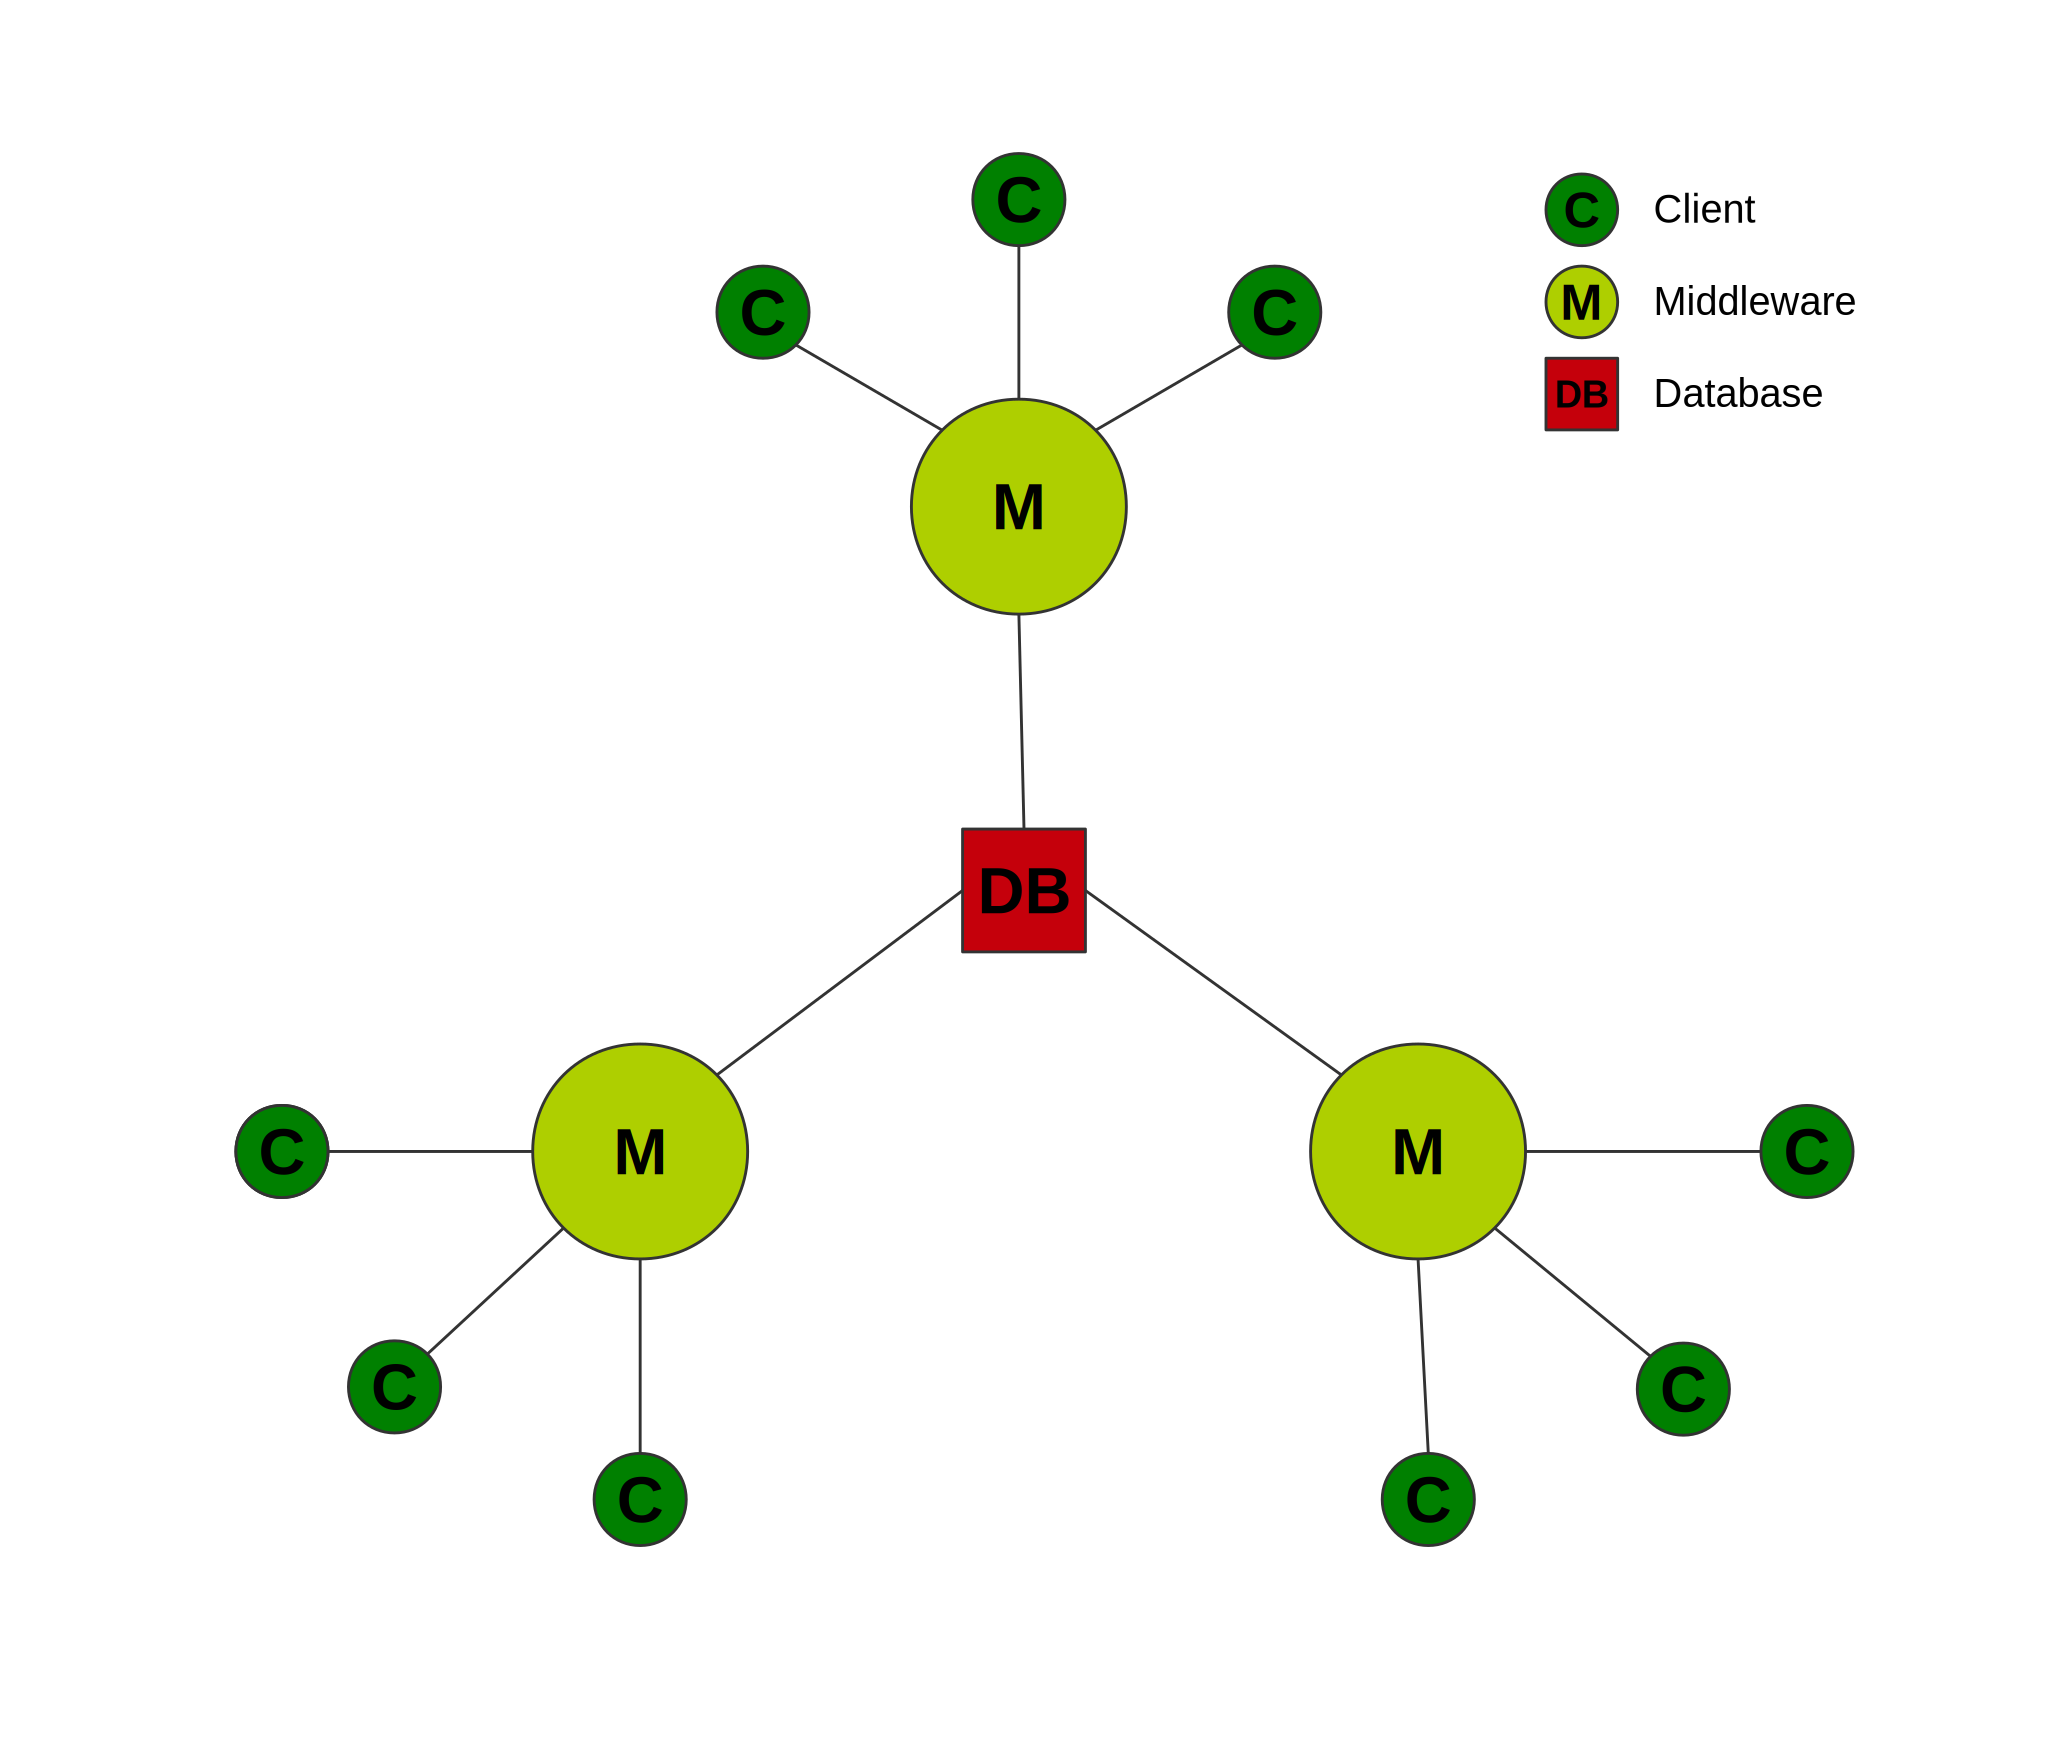
\includegraphics[width=0.9\textwidth]{architecture-new}
            \caption{Sample architecture diagram of \telesto{} with $3$
            middlewares each serving $3$ clients and one central database.}
            \label{fig:telesto-architecture}
    \end{figure}

\section{Database}
\label{sec:db}
    
    \telesto{} uses {\it PostgreSQL} as underlying database. It comes with a lot
    of features of which only a small subset are actually used by \telesto. The
    main directive for building the database was focusing on a simple and
    scalable design and using stored procedures to do all database interactions
    rather than prepared statements. The latter reduces the use of {\it SQL} in
    the middleware to an absolute minimum since only function calls have to be
    passed to the database.
    
\subsection{Entities}
    In \telesto{} there exist only three different entities:
    
    \begin{description}
    \item[Client] \ \\
        A client to the system identified by a unique name and client\_id.
        Clients have a certain mode indicating whether they are only allowed to
        read messages or also put new ones.
    \item[Queue] \ \\
        A queue that can contain multiple messages and is identified by a unique
        name and queue\_id
    \item[Message] \ \\
        A string message in exactly one queue with a client as sender, a
        potential receiver, a priority, a content string and, if the message is
        part of a request response interaction, a context. Additionally a
        timestamp is stored indicating when the message arrived in the system.
    \end{description}

    \begin{table}[t]
        \centering
        \rowcolors{1}{Gray}{white}
        \begin{tabular}{$l^c^r}
            \rowcolor{DarkGray}
            \rowstyle{\bfseries}
            Field name & type & Description\\
            \hline
            client\_id & serial & primary key using sequence \\
            client\_name & varchar(255) & unique \\
            client\_mode & smallint & \\
        \end{tabular}
        \caption{Table {\tt clients}}
        \label{tbl:db-clients}
    \end{table}
    
    \begin{table}[t]
        \centering
        \rowcolors{1}{Gray}{white}
        \begin{tabular}{$l^c^r}
            \rowcolor{DarkGray}
            \rowstyle{\bfseries}
            Field name & type & Description\\
            \hline
            queue\_id & serial & primary key using sequence \\
            queue\_name & varchar(255) & unique \\
        \end{tabular}
        \caption{Table {\tt queues}}
        \label{tbl:db-queues}
    \end{table}
    
    \begin{table}[b]
        \centering
        \rowcolors{1}{Gray}{white}
        \begin{tabular}{$l^c^r}
            \rowcolor{DarkGray}
            \rowstyle{\bfseries}
            Field name & type & Description\\
            \hline
            message\_id & serial & primary key using sequence \\
            queue\_id & integer &  \\
            sender\_id & integer & \\
            receiver\_id & integer & \\
            context & integer & \\
            priority & smallint & between $1$ (lowest) and $10$ \\
            time\_of\_arrival & timestamp & set to {\tt now()} by default \\
            message & varchar(2000) & the actual message \\
        \end{tabular}
        \caption{Table {\tt messages}}
        \label{tbl:db-messages}
    \end{table}

    Each of this entities can directly be modeled into one database table each
    as shown in \cref{tbl:db-clients,tbl:db-queues,tbl:db-messages}.

    In order to create the tables we used {\it PgAdmin 3}\websource{pgAdmin
    Website}{http://www.pgadmin.org/}{November 15, 2013} on a local
    development database and used the backup function to create a dump which
    could be distributed to our testing environment.
    
    We deliberately pass on creating foreign key constraints on our tables
    because 
    \begin{inparaenum}[\itshape a\upshape)]
        \item we use table joins for just one operation (i.e. {\tt
        get\_active\_queues()}, see \cref{sec:stored-procedures}) which can also
        be handled by an index; 
        \item we don't need any actions on update or deletion except for the
        case when a queue is deleted, which can easily be handled individually;
        \item we are sure that we don't insert inconsistent data because data is
        never updated~\footnote{There is actually no support to change queue or
        client names. This could however be added while still not rendering this
        argument invalid because only id rather than name attributes would be
        used as foreign keys} and queue existence is checked on insert; and
        \item we support inserting messages for not (yet) existing clients by
        design because they may only register themself at a later point in time.
    \end{inparaenum}

\subsection{Indexes}
    The main actions on the database in \telesto{} are inserting messages and
    removing them (by reading them). Since reading messages supports some
    parameters (see \cref{tbl:query-params}), it is strongly recommended to use
    appropriate indexes on the affected tables. Additionally to the indexes
    specifically introduced to optimize the performance of a selection or
    sorting operation for message finding, there are primary keys indexed on
    every table which lower the cost of getting entries directly by their id.
    
\begin{table}[t]
    \centering
    
    \begin{adjustbox}{center}
        \rowcolors{1}{Gray}{white}
        \begin{tabular}{$l^c^c^p{5cm}}
            \rowcolor{DarkGray}
            \rowstyle{\bfseries}
            Parameter & affected fields & required & Description\\
            \hline
            queue\_id & queue\_id & X &  \\
            receiver\_id & receiver\_id & X & matches if either {\tt null} or own
            client\_id \\
            sender\_id & sender\_id &  &  \\
            context & context &  & to identify responses \\
            mode & priority, time\_of\_arrival & X & one of both used for ordering
            \\
            
        \end{tabular}
    \end{adjustbox}
    \caption{Parameters of a message query}
    \label{tbl:query-params}
\end{table}

    Based on the data from \cref{tbl:query-params} we decided only use
    multi-column indexes for the table {\tt messages} that always include the
    {\tt receiver\_id} as first part and the {\tt queue\_id} as second. The {\tt
    receiver\_id} is either an integer value or {\tt null}. In both cases the
    query executor should be able to use the second part, namely the {\tt
    queue\_id} which is always present. The details of each separate index are
    listed below:
    
    \begin{description}
    \item[receiver\_id, queue\_id, priority] \ \\
        For a query by priority and without specified sender
    \item[receiver\_id, queue\_id, priority, sender] \ \\
        For a query by priority with specified sender
    \item[receiver\_id, queue\_id, time\_of\_arrival] \ \\
        For a query by time without specified sender
    \item[receiver\_id, queue\_id, time\_of\_arrival, sender] \ \\
        For a query by time with specified sender
    \end{description}

\subsection{Stored Procedures}
\label{sec:stored-procedures}

    As mentioned above, all database interaction is done using stored
    procedures\websource{PostgreSQL 9.3 
    Documentation: SQL Procedural Language
    }{http://www.postgresql.org/docs/9.3/static/plpgsql.html}{November 15,
    2013}\websource{PostgreSQL 9.3 Documentation: CREATE
    FUNCTION}{http://www.postgresql.org/docs/9.3/static/sql-createfunction.html}{November
    15, 2013}. For most of the database functions we used the standard {\it SQL}
    language syntax rather than the special {\it PL/pgSQL} language because the
    simple version serves almost all our requirements and it is often possible
    to write very easy queries in a very simple way. We however did not test if
    queries would run faster using {\it PL/pgSQL} because of the additional
    options {\it PostgreSQL} offers for these stored
    procedures.\websource{Advantages of Using PL/pgSQL in the official
    documentation
    }{http://www.postgresql.org/docs/9.3/static/plpgsql-overview.html\#PLPGSQL-ADVANTAGES}{November 15, 2013}

    \Cref{tbl:procedures} lists all implemented stored procedures in
    the database of \telesto.
    They very directly resemble the methods supported by our network protocol
    (see \cref{sec:protocol}) which means there is not much logic required on
    the middleware in order to execute a query on the database given a request
    packet.
    
    To simplify the database abstraction in the middleware we tried to produce
    very consistent return values. All functions either return tables of Queues,
    Messages, Clients or single integers. (where many are constrained to a
    single entry) For error handling, unique constraint violations are detected
    by the middleware and both {\tt put\_message} and {\tt put\_messages} return
    the {\tt queue\_ids} of the queues successfully inserted to (an id might be
    missing if the queue did not exist). Like this, errors from the database can
    be transformed into an appropriate {\tt ErrorPacket} as introduced in the
    next section.

\begin{table}[hp]
    \centering
    
    \begin{adjustbox}{center}
        \rowcolors{1}{Gray}{white}
        \begin{tabular}{$l^l^c^p{5cm}}
            \rowcolor{DarkGray}
            \rowstyle{\bfseries}
            Name & Parameters & Return Value & Description\\
            \hline

            \rowcolor{DarkGray}
            \multicolumn{4}{c}{Client Manipulation} \\
            \hline
            request\_id & 
            \parbox[t]{2.5cm}{client\_name,\\ mode} 
            & client\_id & create
            a new client \\
            identify & client\_id & Client & identify a client \\
            delete\_client & client\_id & client\_id & delete a client \\
            
            \hline
            \rowcolor{DarkGray}
            \multicolumn{4}{c}{Queue Manipulation} \\
            \hline
            create\_queue & queue\_name & Queue & creates a new queue \\
            delete\_queue & queue\_id & queue\_id & delete a queue \\
            get\_queue\_id & queue\_name & Queue & get queue by name \\
            get\_queue\_name & queue\_id & Queue & get queue by id\\
            list\_queues &  & array[Queue] & get all queues \\
            
            get\_active\_queues & client\_id & array[Queue] & get all queues with
            messages for the given client \\
            get\_messages\_from\_queue & queue\_id & array[Message] & get all
            message in a queue \\
            
            \hline
            \rowcolor{DarkGray}
            \multicolumn{4}{c}{Message Manipulation} \\
            \hline
            put\_message & 
            \parbox[t]{2.5cm}{queue\_id,\\ sender\_id,\\ receiver\_id,\\
            context,\\
            priority,\\ message}
             & queue\_id & insert message and return queue
            \\
            
            put\_messages & 
            \parbox[t]{2.5cm}{array[queue\_id],\\ sender\_id,\\ receiver\_id,\\
            context,\\
            priority,\\ message}
             & array[queue\_id] & insert messages in multiple queues and return
             queues
            \\
            
            read\_message\_by\_priority & 
            \parbox[t]{2.5cm}{queue\_id,\\ sender\_id,\\ receiver\_id}
             & Message & get a message by priority
            \\
            
            read\_message\_by\_timestamp & 
            \parbox[t]{2.5cm}{queue\_id,\\ sender\_id,\\ receiver\_id}
             & Message & get a message by timestamp
            \\
            
            read\_response\_message & 
            \parbox[t]{2.5cm}{queue\_id,\\ receiver\_id,\\ context}
             & Message & get a message by receiver and context
            \\
            
            
            
        \end{tabular}
    \end{adjustbox}
    \caption{Parameters of a message query}
    \label{tbl:procedures}
\end{table}

\section{Network Protocol}
\label{sec:protocol}

    In order to achieve high throughput and low latency, it is essential to have
    a lightweight communication protocol as a foundation. \telesto{} uses a binary
    protocol based on TCP to do all the communication between clients and
    middlewares. Connections to the database are handled by the {\it PostgreSQL
    JDBC Driver}~\websource{PostgreSQL JDBC
    Driver}{http://jdbc.postgresql.org/}{November 15, 2013} which is based on
    TCP as well but isn't part of \telesto{} itself. This section gives insight
    about the network protocol introduced by \telesto{} for the communication
    between clients and middleware.
    
    A middleware offers a certain set of services (i.e methods) to the clients,
    like putting a message in a queue or reading a message from a queue. Every
    such method is identified by a special {\tt method id}. All method calls and
    responses are grouped into one \telesto{} packet consisting of four parts:
    \begin{description}
    \item[length] \ \\
        The length of the entire packet in bytes. This value is sent as a {\tt
        short} type integer which allows values of up to $32,768$. This limits
        the packet size, which is fine since the maximum supported message size
        is $2000$ characters and all other fields are a lot smaller. Only the
        method to read all messages from a queue might (in rare cases) try to
        serve more data which would then fail.
    \item[method id] \ \\
        A {\tt short} containing the method id in order to identify the service
        requested and how to interpret the payload.
    \item[client packet\_id] \ \\
        An id that is set by the client and repeated by the middleware in the
        associated response in order to identify which request yielded which response.
    \item[payload] \ \\
        The varying length payload containing all the arguments of the method
        call or the structured response data.
    \end{description}
    
     Figure \TODO{add
    protocol figure} shows the basic structure of such a packet.
    
    Besides a packet for each method call, there is one for the according
    response if applicable and two additional packets named {\tt SuccessPacket}
    and {\tt ErrorPacket} to indicate a successful call of a method with no
    return value or an error during execution respectively.
    
    By convention the {\tt packet id} for a response is always higher by one
    than the according request. A complete list of the currently supported methods and
    their parameters is shown in \cref{tbl:packets}.
    
    \begin{table}[hp]
        \centering
        \begin{tabular}{$l^c^r}
            \rowcolor{DarkGray}
            \rowstyle{\bfseries}
            Packet & method\_id & payload\\
            \hline
            Ping & 0x01 & \\
            Pong & 0x02 & \\
            Success & 0x03 & \\
            Error & $0x05$ & error\_type\\
            \hline
            \rowcolor{Gray}
            \multicolumn{3}{c}{Client Manipulation} \\
            \hline
            RegisterClient & 0x11 & client\_name, mode\\
            RegisterClientResponse & 0x12 & client\_id\\
            IdentifyClient & 0x13 & client\_id\\
            IdentifyClientResponse & 0x14 & mode, client\_name\\
            DeleteClient & 0x15 & client\_id\\
            \hline
            \rowcolor{Gray}
            \multicolumn{3}{c}{Queue Manipulation} \\
            \hline
            CreateQueue & 0x21 & queue\_name\\
            CreateQueueResponse & 0x22 & queue\_id\\
            DeleteQueue & 0x23 & queue\_id\\
            GetQueueId & 0x25 & mode, queue\_name\\
            GetQueueIdResponse & 0x26 & queue\_id\\
            GetQueueName & 0x27 & queue\_id\\
            GetQueueNameResponse & 0x28 & queue\_name\\
            GetQueues & 0x29 & \\
            GetQueuesResponse & 0x2a & array[Queue]\\
            GetActiveQueues & 0x2b & \\
            GetActiveQueuesResponse & 0x2c & array[Queue]\\
            GetMessages & 0x2d & queue\_id\\
            GetMessagesResponse & 0x2e & array[Message]\\
            \hline
            \rowcolor{Gray}
            \multicolumn{3}{c}{Message Manipulation} \\
            \hline
            PutMessage & 0x31 & Message, array[queue\_id]\\
            ReadMessage & 0x32 & queue\_id, sender\_id, mode\\
            ReadMessageResponse & 0x33 & array[Message]\\
            ReadResponse & 0x34 & queue\_id, context\\
        \end{tabular}
        \caption{Supported packets in \telesto. By convention an odd {\tt
        method\_id} indicates client to server communication while even values
        are server to client communication. Queue and Message objects in the
        payload include all fields stored in the database (see \cref{sec:db}).
        The {\tt mode} in the ReadMessage packet is used to indicate whether
        the oldest message or the one with the highest priority should be
        served.}
        \label{tbl:packets}
    \end{table}
    
    By using this lightweight binary packet format, the overall packet size is
    only slightly larger than a binary sequence of all input parameters of a
    method which is certainly a good prerequisite for handling high loads with
    many requests in short time. 
    %As seen in \cref{ch:evaluation}, the load on the network was never a
    % problem during performance tests.


\section{Middleware}

    The middleware is the core part of \telesto{} as it serves incoming request
    from clients in a highly efficient manner. The tasks arising can be split in
    $4$ parts:
    
    \begin{enumerate}
        \item Handling incoming connections and data
        \item Parsing the request packet
        \item Executing the according database action
        \item Sending back a response
    \end{enumerate}

    Using asynchronous Java {\tt
    nio}\websource{Java
    Documentation:
    java.nio}{http://docs.oracle.com/javase/7/docs/api/java/nio/package-summary.html}{November
    15, 2013}, it is possible to handle a lot of concurrent connections to
    multiple clients simultaneously in an efficient manner. A single
    dispatcher thread handles new incoming connections and data by putting
    the clients into a FIFO queue which is continuously worked off by multiple
    worker threads. The actual parsing, database action and response sending is done by
    a worker rather than the dispatcher in order to reduce the load on the
    dispatcher.
    
    In order to interact with the database, a database connection pool is used
    with a limited number of connections. Workers can request a connection from
    this pool, execute their queries and then put the connection back for other
    workers to use.
    
    \Cref{fig:middleware} shows an overview of the three main parts in the
    middleware; namely the dispatcher, the worker threads and the database
    connection pool.
    
    It is important to note, that connections to clients are never closed by the
    middleware (unless on shutdown). This first improves the delay of the
    system because no new TCP connection establishment is necessary for each
    request and second it allows to store the client information together with
    the connection so it is never necessary to send the {\tt client\_id} to the
    middleware again after the initial identification. This is the reason, why
    every client is first only allowed to request a limited set of services
    because many of them require identification. These services are namely the
    client registration and identification, and the pinging system.

    \begin{figure}[ht]
        \centering
            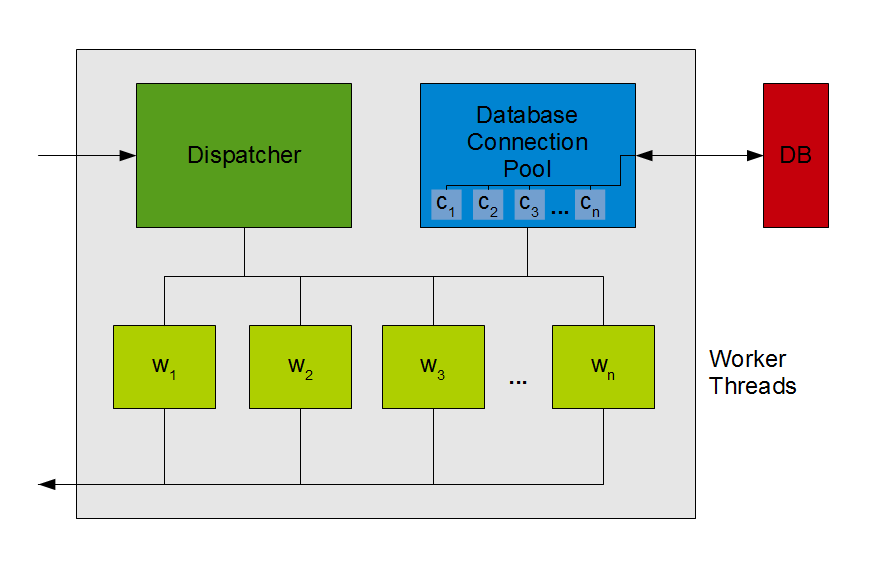
\includegraphics[width=0.9\textwidth]{middleware}
            \caption{Basic setup of a middleware instance including the
            dispatcher, multiple worker threads and a database connection pool.}
            \label{fig:middleware}
    \end{figure}


\section{Client}
    \telesto{} offers a simple interface for clients that want to use the system.
    The actual public Application Programming Interface (API) consists of one
    simple class {\tt TelestoClient} with all the offered functionality. It is
    as easy as creating a new instance and then start calling functions to
    actually use \telesto.
    
    By design, a client is only allowed to do further actions if he either
    registered itself as a new client or identified itself using his client id.
    This means, the first API call has to be to the {\tt connect()} or method
    supplying either an existing {\tt client\_id} or both a new name and the
    mode of the client. (or {\tt ping()} which is always allowed)
    
    The API works in a synchronous way and has some blocking functions that
    retry an operation with a certain (configurable) delay until successful. An
    example of this is requesting a message from a queue, which blocks until a
    message for the client is successfully read.
    
    It would be possible to actually build a client implementation that is
    asynchronous since the middleware and the used protocol support that
    feature. However we went without such an implementation as the testing of
    the system is in many cases much easier when using synchronous clients.
    

\chapter{Implementation}
\label{ch:implementation}
This chapter gives more detailed overview of some decisions made during the
implementation phase of \telesto. This is a good starting point before getting
involved with the code base of the system as it gives the necessary orientation
and overview.


\section{Networking}
    In order to make networking efficient and fast, it is essential that
    involved parts of the system are never a bottleneck to the entire system
    performance.
    
\subsection{Packet parsing}


\section{Database Interaction}


\section{Client}
    \Cref{tbl:client-api} shows a brief overview of the offered
    functionality by the \telesto{} client API. A more detailed description of
    each method is available inside the class {\tt
    ch.ethz.syslab.telesto.client.TelestoClient} as {\it
    javadoc}\websource{Oracle:
    How to Write Doc Comments for the Javadoc Tool
    }{http://www.oracle.com/technetwork/java/javase/documentation/index-137868.html}{November 15, 2013}.
    
    \begin{table}[p]
        \centering
        
        \begin{adjustbox}{center}
            \rowcolors{1}{Gray}{white}
            \begin{tabular}{$l^l^c^p{4cm}}
                \rowcolor{DarkGray}
                \rowstyle{\bfseries}
                Method & Parameters & Return Value & Description \\
                \hline
                \rowcolor{DarkGray}
                \multicolumn{4}{c}{Setup} \\
                \hline
                
                ping & & round trip time & ping the middleware \\
                connect & 
                \parbox[t]{2.5cm}{clientName,\\ clientMode} & Client & connect
                to the middleware as new client  \\
                connect & clientId & Client & connect to the middleware as
                existing client \\
                
                \hline
                \rowcolor{DarkGray}
                \multicolumn{4}{c}{Queues} \\
                \hline
                createQueue & queueName & Queue & create a new queue \\
                deleteQueue & queueId &  & delete a queue \\
                getQueueByName & queueName & Queue & get a queue by its name \\
                getQueueById & queueId & Queue & get a queue by its id \\
                getQueues &  & List\textless Queue\textgreater & get all queues \\
                getActiveQueues &  & List\textless Queue\textgreater & get all queues with messages
                for this client \\
                readMessages & queueId & List\textless Message\textgreater & get
                all messages from a queue
                \\
                
                \hline
                \rowcolor{DarkGray}
                \multicolumn{4}{c}{Messages} \\
                \hline
                putMessage & Message &  & insert a new message \\
                putMessages & 
                \parbox[t]{2.5cm}{Message,\\ queueId[]} &  & insert a new
                message into multiple queues \\
                sendRequestResponseMessage & Message & Message & send request
                and retrieve response
                \\
                retrieveMessage & queueId & Message & get message from queue
                by priority \\
                retrieveMessage & 
                \parbox[t]{2.5cm}{queueId,\\ readMode} & Message & get message
                from queue by the indicated readMode
                \\
                retrieveMessage & 
                \parbox[t]{2.5cm}{queueId,\\ senderId,\\ readMode} & Message &
                get message from specific sender from queue by the indicated
                readMode
                \\
                retrieveMessage & 
                \parbox[t]{2.5cm}{queueId,\\ senderId,\\ readMode} & Message &
                get message from specific sender from queue by the indicated
                readMode
                \\
                
            \end{tabular}
        \end{adjustbox}
        \caption{Public methods on the {\tt TelestoClient} class. The class is
        also fully documented using {\it javadoc} in order to allow for
        easy usage.}
        \label{tbl:client-api}
    \end{table}

\section{Error Handling}



\chapter{Evaluation and Analysis}
\label{ch:evaluation}

\section{Setup}

\section{Parameters}

\section{Metrics}

\section{Tests}

\subsection{Scalability}
\subsection{Stability}


    \begin{figure}[htbp]
        \centering
        \begin{minipage}[t]{0.45\textwidth}
            \centering
            \includegraphics[width=0.9\textwidth]{jukefox-explore-album-list-1.png}
            \caption{The album list containing suggested albums.}
            \label{fig:album_list1}
        \end{minipage}
        \begin{minipage}[t]{0.45\textwidth}
            \centering
            \includegraphics[width=0.9\textwidth]{jukefox-streamplayer1}
            \caption{The jukefox music streaming view.}
            \label{fig:stream_player}
        \end{minipage}
    \end{figure}

\chapter{Future Work}
	
\section{Possible Improvements}

\chapter{Conclusion}

	

% This displays the bibliography for all cited external documents. All references have to be defined in the file references.bib and can then be cited from within this document.
\bibliographystyle{splncs}
\bibliography{references}

% This creates an appendix chapter, comment if not needed.
\appendix
\chapter{Appendix Chapter}

\section{Database Structure}

	
\end{document}